\textbf{2-1} 如力图2-1-1，在固定不动的圆柱体上绕有绳索，绳两端挂大、小两桶，其质量分别为 $M = 1000\,\mathrm{kg}$ 和 $m = 10\,\mathrm{kg}$。绳与圆柱体之间的摩擦系数为 $\mu = 0.050$，绳的质量可以忽略。试问为使两桶静止不动，绳至少需绕多少圈。

\begin{center}
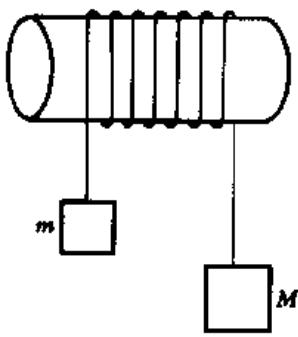
\includegraphics[width=0.15\textwidth]{figures/力图2-1-1.jpg}
\end{center}
\vfill

\textbf{2-2} 如力图2-2-1，细杆一端支在地面上，以恒定的角速度 $\omega$ 绕通过支点的竖直轴旋转，杆与地面的夹角为 $\alpha$，质量为 $m$ 的小环套在杆上，可以沿杆滑动，环与杆之间的摩擦系数为 $\mu$。试问小环处于什么位置上能维持稳定运动。

\begin{center}
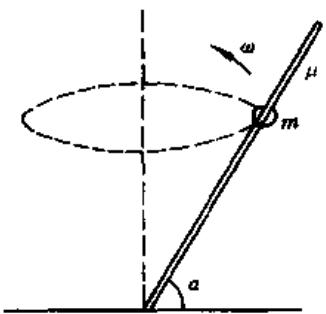
\includegraphics[width=0.15\textwidth]{figures/力图2-2-1.jpg}
\end{center}
\vfill
\newpage

\textbf{2-3} 如力图2-3-1，在半径为 $R$ 的空心球壳内壁，有一可当作质点的小球沿固定的水平圆周作匀速率运动，小球与空心球壳球心的连线与铅垂线的夹角为 $\theta$，小球与空心球壳内壁之间的摩擦系数为 $\mu$。试求小球能稳定运动的速度范围。

\begin{center}
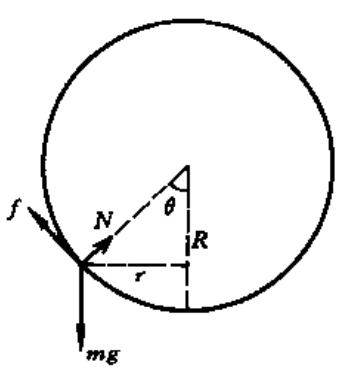
\includegraphics[width=0.15\textwidth]{figures/力图2-3-1.jpg}
\end{center}
\vfill


\textbf{2-4} 如力图2-4-1，在地面上有一倾角为 $\theta$、质量为 $M$ 的斜面体，斜面体上有一质量为 $m$ 的木块，设地面与斜面体之间以及斜面体与木块之间均光滑无摩擦。试求 $M$ 与 $m$ 相对于地面的加速度 $a_{M}$ 与 $a_{m}$，以及木块 $m$ 所受的支持力。

\begin{center}
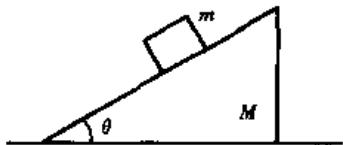
\includegraphics[width=0.3\textwidth]{figures/力图2-4-1.jpg}
\end{center}
\vfill

\newpage

\textbf{2-5} 如力图2-5-1，一个半径为 $R = 0.5\,\mathrm{m}$ 的空心球壳绕本身的竖直直径旋转，角速度为 $\omega = 5\,\mathrm{s^{-1}}$，在空心球壳内高度为 $\dfrac{R}{2}$ 处有一小木块（可当作质点）同球壳一起旋转。

试求：1. 摩擦系数至少是多少才能实现这一情况。2. 当 $\omega = 8\,\mathrm{s^{-1}}$ 时，实现这一情况的条件是什么。3. 研究以下两种情形运动的稳定性：(a) 木块位置有微小变动；(b) 空心球壳的角速度有微小变动。

\begin{center}
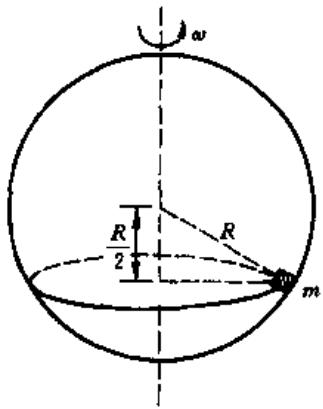
\includegraphics[width=0.15\textwidth]{figures/力图2-5-1.jpg}
\end{center}
\vfill

\textbf{2-6} 如力图2-6-1，一质量为 $m = 20\,\mathrm{kg}$ 的对称钢件，架在两个完全相同的平行长直滚轴上。两滚轴在同一水平面内，滚轴半径为 $r = 0.025\,\mathrm{m}$，绕各自的中心轴以相同的角速度 $\omega = 40\,\mathrm{rad/s}$ 作反向转动。钢件与滚轴间的摩擦系数为 $\mu = 0.20$。为使钢件以 $v_{0} = 0.050\,\mathrm{m/s}$ 的速度沿滚轴作匀速直线运动，需沿滚轴的长度方向对钢件施以水平作用力 $F$，试求 $F$ 的大小。

\begin{center}
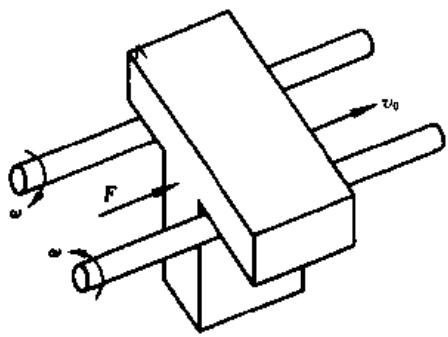
\includegraphics[width=0.15\textwidth]{figures/力图2-6-1.jpg}
\end{center}
\vfill

\newpage

\textbf{2-7} 如力图2-7-1所示，质量分别为 $m_{A}$ 和 $m_{B}$ 的两木块 A 和 B 静止放置在粗糙的水平地面上，两者与地面之间的摩擦系数均为 $\mu$，两木块 A 和 B 的接触面是倾角为 $\theta$ 的斜面，接触面是光滑的。现施一水平推力 $F$ 于 A，使 A 和 B 产生向右的加速度，且 A 和 B 之间不发生相对滑动。试问 $\mu$ 和 $F$ 各应满足什么条件。

\begin{center}
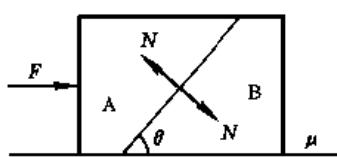
\includegraphics[width=0.2\textwidth]{figures/力图2-7-1.jpg}
\end{center}
\vfill

\textbf{2-8} 如力图2-8-1所示，质量为 $M$ 的滑块C放置在光滑桌面上。质量均为 $m$ 的两个重物 A 和 B 用细绳相连，A 平放在滑块上，与滑块间的摩擦系数为 $\mu$，细绳跨过滑轮后将 B 竖直悬挂。设细绳和滑轮的质量均忽略不计，滑轮转轴不受摩擦力。今以水平推力 $F$ 作用于滑块，为使重物 A 和 B 与滑块保持相对静止，试问 $F$ 至少应多大？

\begin{center}
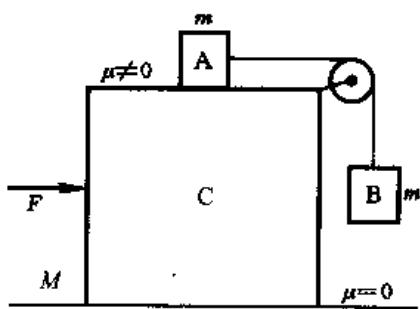
\includegraphics[width=0.2\textwidth]{figures/力图2-8-1.jpg}
\end{center}
\vfill

\newpage

\textbf{2-9} 如力图2-9-1所示，在水平面内有一平台可绕竖直的中心轴以角速度 $\omega$ 匀角速旋转，在平台内沿半径方向有一光滑细槽，槽内放置两质量均为 $m$ 的小球，两球用劲度系数为 $k$、原长为 $a$ 的轻弹簧相连。弹簧的自然长度恰好等于槽的宽度，即两球刚好接触。平台以角速度 $\omega$ 旋转时，两球在槽内离中心的距离分别为 $r_{1}$ 和 $r_{2}$，试求 $r_{1}$ 和 $r_{2}$。

\begin{center}
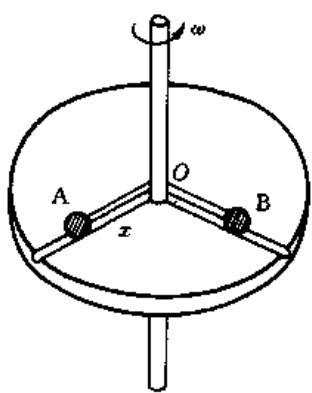
\includegraphics[width=0.2\textwidth]{figures/力图2-9-1.jpg}
\end{center}
\vfill



\textbf{2-10} 质量为 $m$ 的物体以初速 $v_{0}$ 从地面竖直上抛，设空气阻力 $f = \mu v^{2}$，$\mu$ 为常数。试求物体达到的最大高度，并证明物体返回原处的速度为 $v_{0}\sqrt{\dfrac{mg}{mg + \mu v_{0}^{2}}}$。

\vfill

\newpage

\textbf{2-11} 两质点的质量均为 $m$，质点1从离地面高度为 $h$ 处由静止下落，质点2从质点1正下方的地面上以初速 $v_0$ 同时竖直上抛。设空气阻力与质点速率成正比，比例系数为 $\mu$（常量）。试求两质点相遇的时间、地点以及相遇时两质点的速度。

\vfill

\textbf{2-12} 质量为 $m$ 的抛射体初速为 $v_{0}$，抛射角为 $\alpha$，在空气中运动时，所受阻力与速率成正比，比例系数为 $k$。试求轨迹方程，并验证当 $k \to 0$ 时变为抛物方程。

\vfill

\newpage

\textbf{2-13} 飞机以 $v_{0} = 90\,\mathrm{km/h}$ 的水平速度触地滑行着陆。滑行期间受到的空气阻力为 $c_{x}v^{2}$，升力与速度平方成正比，即 $L = c_{y}v^{2}$。已知飞机质量为 $m$，机翼面积为 $S$，升阻比 $K = \dfrac{c_y}{c_x} = 5$，触地瞬间升力与重力恰好平衡。试求飞机触地后的滑行距离 $x$ 和速度随时间的变化关系 $v(t)$。

\vfill

\textbf{2-14} 如力图2-14-1，质量为 $m$ 的小球用一质量可略的弹簧1竖直悬挂起来，弹簧的劲度系数为 $k$。当弹簧的伸长量超过临界长度 $l_{\mathrm{C}}$ $\left(l_{\mathrm{C}} > \dfrac{mg}{k}\right)$ 时，弹簧将被拉断。在小球下方再挂完全相同的另一弹簧2，并在其下端施一与时间 $t$ 有关的拉力 $F(t)$。若以小球在平衡位置时作为计时起点，则拉力随时间变化的关系为 $F(t) = \alpha t$，其中 $\alpha$ 是一恒定参量。试求两弹簧同时被拉断时，参量 $\alpha$ 应满足的关系式。

\begin{center}
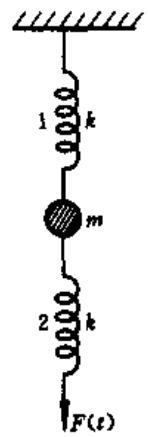
\includegraphics[width=0.08\textwidth]{figures/力图2-14-1.jpg}
\end{center}
\vfill

\newpage

\textbf{2-15} 如力图2-15-1，质量为 $M$、倾角为 $\theta$ 的斜面体放在光滑的桌面上，斜面体上有质量为 $m$ 的木块，木块与斜面体之间的摩擦系数 $\mu < \tan \theta$，以水平力 $F$ 推斜面体，使之运动。试问为了使木块相对于斜面体保持静止，$F$ 的大小应在什么范围。

\begin{center}
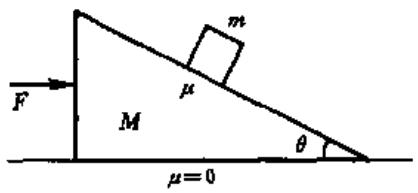
\includegraphics[width=0.25\textwidth]{figures/力图2-15-1.jpg}
\end{center}
\vfill

\textbf{2-16} 如力图2-16-1，地面上有一质量为 $M$、倾角为 $\alpha_{1}$、$\alpha_{2}$ 的斜面体。质量为 $m_{1}$ 和 $m_{2}$ 的两木块分别置于斜面体两侧，用绳经滑轮相连。设地面、斜面、滑轮的摩擦以及绳子和滑轮的质量均可忽略，绳不可伸长，试求 $m_{1}$（或 $m_{2}$）相对 $M$ 的加速度以及 $M$ 的绝对加速度。

\begin{center}
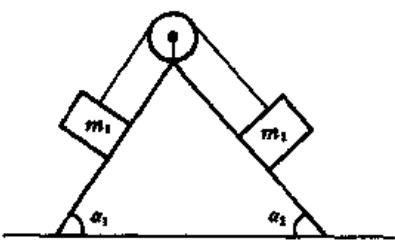
\includegraphics[width=0.25\textwidth]{figures/力图2-16-1.jpg}
\end{center}
\vfill

\newpage

\textbf{2-17} 如力图2-17-1，质量为 $m_{1}$ 的航天飞机A绕地球作匀速圆周运动，轨道半径为 $R$，从航天飞机伸出一长度为 $L$ $(L \ll R)$ 的刚性杆，杆端固定一质量为 $m_{2}$ $(m_{2} \ll m_{1})$ 的卫星S。设A和S均可看作质点，A-S系统的位置用 $\alpha$ 角表示，$\alpha$ 角是杆与A和地心连线之间的夹角。试求A-S系统的平衡位置，并讨论平衡的稳定性。

\begin{center}
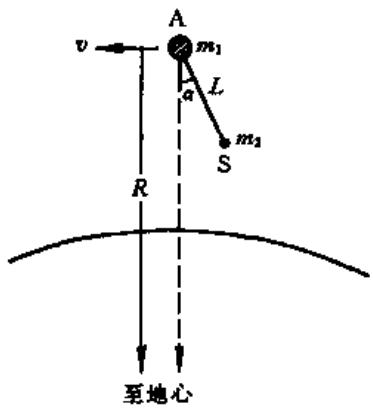
\includegraphics[width=0.2\textwidth]{figures/力图2-17-1.jpg}
\end{center}
\vfill

\textbf{2-18} 如力图2-18-1，半径为 $R$ 的圆盘与水平面平行，绕通过盘中心 $O$ 的竖直轴以角速度 $\omega$ 匀速旋转。盘边缘 $A$ 点处的射手相对于圆盘以水平初速 $v_{0}$ 发射子弹，目标是直径 $AB$ 的另一端点 $B$。设子弹速度远大于盘的转速，且发射子弹不影响圆盘的角速度，设空气阻力可忽略。试问射手应瞄准何方才能击中目标？从射手看来，子弹的轨迹如何？

\begin{center}
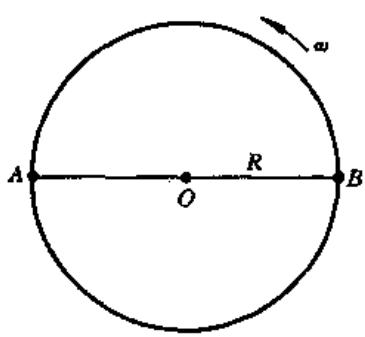
\includegraphics[width=0.2\textwidth]{figures/力图2-18-1.jpg}
\end{center}
\vfill

\newpage

\textbf{2-19} 地球以角速度 $\omega$ 自转，一质点在纬度 $\varphi$ 上空 $h$ 高度处自由下落。忽略空气阻力和惯性离心力。试求因科里奥利力引起的落地点的偏离。

\vfill

\textbf{2-20} 1851年，法国物理学家傅科发现单摆并不在固定的平面内摆动。如果把每次摆动近似看作在一个平面内，并把这个平面称为摆动平面，则摆动平面将以一定角速度作缓慢的顺时针转动（在北半球）。这个现象是由地球的自转造成的，这种摆称为傅科摆。试证明傅科摆摆动平面的旋转周期 $T'$ 与摆所在处的纬度 $\varphi$ 有关，并遵守

\[
T' = \frac{T_0}{\sin\varphi}
\]

式中 $T_0 = \dfrac{2\pi}{\omega}$ 为地球自转周期。

